\section{Meet Mosaic}
\label{sec:ch01-meet-mosaic}
\index{Mosaic|(}

Books about distributed systems have a habit of teaching mechanisms on toy
schemas where nothing is at stake. A \code{User} with a \code{name}, a
\code{Post} with a \code{title}, an arrow between them, and the hard part
skipped. The hard part is never the arrow. It is that two teams both have a
legitimate claim on the same type, and the schema has to express that claim
without either team asking permission to ship.

So we build one system for the whole book. Mosaic is an online storefront: a
catalog of products, prices that change more often than the products do,
stock levels that change faster still, orders, customer accounts, and reviews.
Retail is a good teacher here because its central noun is genuinely shared.
A product is not owned by one team in any useful sense. Merchandising writes
its description, pricing sets what it costs today, the warehouse knows whether
you can have it, and customers attach opinions to it. Six domains, one noun.

\begin{figure}[htbp]
  \centering
  % Mosaic's six domains inside one deployable, with the seams the book later
% cuts along. Referenced from chapter 01. Bare tikzpicture; the figure
% environment, caption and label live at the call site.
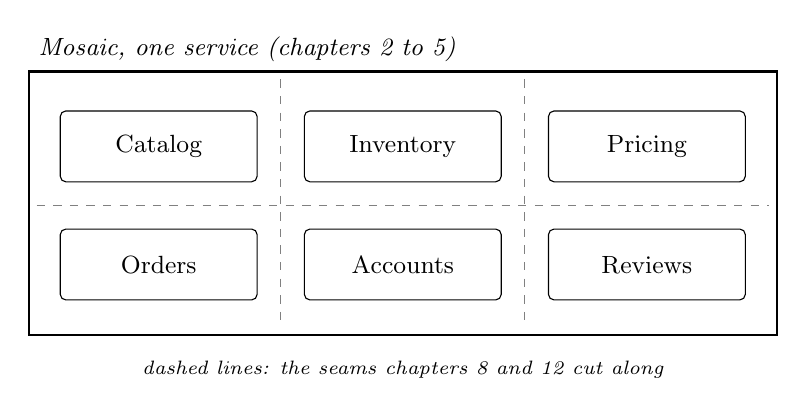
\begin{tikzpicture}[
    font=\small,
    dom/.style={draw, rounded corners=2pt, minimum width=25mm,
                minimum height=9mm, align=center},
    seam/.style={dashed, gray},
    note/.style={font=\scriptsize\itshape, align=center}
  ]

  \node[dom] (cat) at (0,0)      {Catalog};
  \node[dom] (inv) at (3.1,0)    {Inventory};
  \node[dom] (pri) at (6.2,0)    {Pricing};
  \node[dom] (ord) at (0,-1.5)   {Orders};
  \node[dom] (acc) at (3.1,-1.5) {Accounts};
  \node[dom] (rev) at (6.2,-1.5) {Reviews};

  % The one deployable everything starts inside.
  \draw[thick] (-1.65,0.95) rectangle (7.85,-2.4);
  \node[anchor=south west, font=\small\itshape] at (-1.65,0.95)
    {Mosaic, one service (chapters 2 to 5)};

  % Seams: where chapters 8 and 12 cut.
  \draw[seam] (1.55,0.85) -- (1.55,-2.3);
  \draw[seam] (4.65,0.85) -- (4.65,-2.3);
  \draw[seam] (-1.55,-0.75) -- (7.75,-0.75);

  \node[note, anchor=north] at (3.1,-2.6)
    {dashed lines: the seams chapters 8 and 12 cut along};

\end{tikzpicture}

  \caption{Mosaic starts as one service holding six domains. The dashed lines
  mark the seams the book eventually cuts along, and they are drawn where the
  data has natural owners rather than where the code happens to be
  convenient.}
  \label{fig:ch01-mosaic-domains}
\end{figure}

Chapters~\ref{ch:hotchocolate-quickly} through
\ref{ch:schema-design-that-survives-change} build Mosaic as a single
HotChocolate service on .NET, and build it properly. That word matters. A
federated graph assembled from services that were sloppy on their own is
worse than the monolith it replaced, because you have added a network between
the sloppy parts. Part I is about earning the right to distribute: resolvers
that batch, a schema that can absorb change, pagination that behaves. If you
already write GraphQL services for a living, that part will move quickly.

Here is where the pressure shows up. In the single-service version, Mosaic's
\code{Product} looks roughly like this:

\begin{graphqlsdl}
# Sketch, not code from the companion repo. Product as chapter 5
# leaves it, with all six domains' fields on one type.
type Product {
  id: ID!
  sku: String!
  title: String!
  description: String
  price: Money!
  availableQuantity: Int!
  averageRating: Float
  reviews(first: Int, after: String): ReviewConnection!
}
\end{graphqlsdl}

Nothing here is wrong. As a client-facing contract it is close to ideal: one
type, one query, everything a product page needs. The problem is that eight
fields are the responsibility of four different groups of people, and the
\code{Product} type is now a file all four of them edit. Add a currency to
\code{price} and you have touched the type that the reviews team is also
changing this sprint. That is the coordination cost from
section~\ref{sec:ch01-org-chart} arriving in a specific place, on a specific
line, and it will not be argued away with better process.

Chapter~\ref{ch:the-first-cut-extracting-catalog} takes the first slice,
moving Catalog out into its own subgraph while everything else stays put.
Chapter~\ref{ch:strangling-the-monolith} carves off the rest one domain at a
time, with the old monolith still serving traffic throughout, because that is
how this actually happens outside of books. By Part~VI, Mosaic is running as
a set of independently deployed services behind a router, with tracing that
crosses service boundaries and a CI pipeline that refuses to publish a
subgraph whose schema would break somebody else's query.

Mosaic runs on .NET~10 with HotChocolate~16 throughout, and lives in a
companion repository tagged per chapter, so you can check out the state of the
system at any point in the book rather than reconstructing it.
Appendix~\ref{app:toolchain} covers the setup and gives you a tour of the
repo. The code in this book comes
from that repository and compiles; where you see a fragment labelled as a
sketch, as in the listing above, it is there to make an argument and is not
something you should expect to find in a source file.
\index{Mosaic|)}
